% This work is made available under the terms of the
% Creative Commons Attribution-ShareAlike 4.0 license,
% http://creativecommons.org/licenses/by-sa/4.0/.
%
% Version: $Revision$

\documentclass[a4paper]{book}

\usepackage{wrapfig}
\usepackage{graphicx}
\usepackage{hyperref}
\usepackage{multirow}
\usepackage{scalefnt}
\usepackage{tikz}

% watermark -- for draft stage
\usepackage[firstpage]{draftwatermark}
\SetWatermarkLightness{0.9}
\SetWatermarkScale{5}

% Copyright (c) 2009 by the University of Waikato, Hamilton, NZ. 
% This work is made available under the terms of the 
% Creative Commons Attribution-ShareAlike 4.0 license,
% http://creativecommons.org/licenses/by-sa/4.0/.
%
% Version: $Revision: 5479 $

\newenvironment{tight_itemize}{
\begin{itemize}
  \setlength{\itemsep}{1pt}
  \setlength{\parskip}{0pt}
  \setlength{\parsep}{0pt}}{\end{itemize}
}

\newenvironment{tight_enumerate}{
\begin{enumerate}
  \setlength{\itemsep}{1pt}
  \setlength{\parskip}{0pt}
  \setlength{\parsep}{0pt}}{\end{enumerate}
}

% if you just need a simple heading
% Usage:
%   \heading{the text of the heading}
\newcommand{\heading}[1]{
  \vspace{0.3cm} \noindent \textbf{#1} \newline
}

\newcommand{\icon}[1]{\tikz[baseline=-3pt]\node[inner sep=0pt,outer sep=0pt]{\includegraphics[height=1.1em]{#1}};}


\title{
  \textbf{ADAMS} \\
  {\Large \textbf{A}dvanced \textbf{D}ata mining \textbf{A}nd \textbf{M}achine
  learning \textbf{S}ystem} \\
  {\Large Module: adams-latex} \\
  \vspace{1cm}
  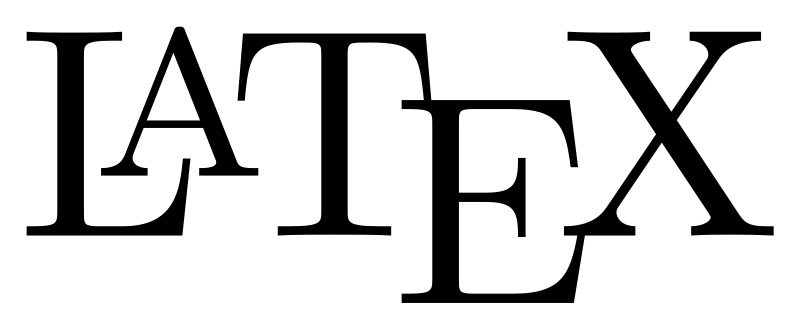
\includegraphics[width=4cm]{images/latex.png} \\
}
\author{
  Peter Reutemann
}

\setcounter{secnumdepth}{3}
\setcounter{tocdepth}{3}

\begin{document}

\begin{titlepage}
\maketitle

\thispagestyle{empty}
\center
\begin{table}[b]
	\begin{tabular}{c l l}
		\parbox[c][2cm]{2cm}{\copyright 2017} &
		\parbox[c][2cm]{5cm}{
\includegraphics[width=5cm]{images/coat_of_arms.pdf}} \\
	\end{tabular}
	
\includegraphics[width=12cm]{images/cc.png} \\
\end{table}

\end{titlepage}

\tableofcontents
\listoffigures
%\listoftables

%%%%%%%%%%%%%%%%%%%%%%%%%%%%%%%%%%%
\chapter{Introduction}
LaTex\cite{latex} is a document preparation system. When writing, the writer
uses plain text as opposed to the formatted text found in WYSIWYG word
processors like Microsoft Word or LibreOffice Writer. The writer uses markup
tagging conventions to define the general structure of a document (such as
article, book, and letter), to stylise text throughout a document (such as
bold and italics), and to add citations and cross-references. A TeX
distribution such as TeX Live or MikTeX is used to produce an output file
(such as PDF or DVI) suitable for printing or digital distribution.

The ADAMS documentation itself is written in LaTeX.

\begin{figure}[htb]
  \centering
  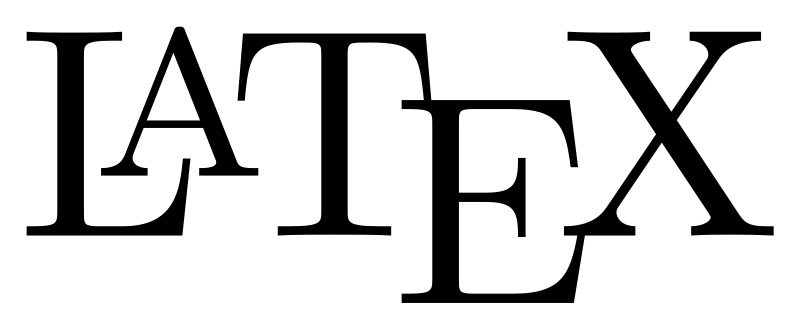
\includegraphics[width=4.0cm]{images/latex.png}
\end{figure}

%%%%%%%%%%%%%%%%%%%%%%%%%%%%%%%%%%%
\chapter{Flow}
The flow comes with a range of actors for accessing the Twitter API.

\noindent The following standalone actors are available:
\begin{tight_itemize}
	\item \textit{LatexSetup} - allows overriding the system-wide
	LaTeX settings.
\end{tight_itemize}

\noindent The following sources are available:
\begin{tight_itemize}
	\item \textit{LatexNewDocument} - generates a new LaTeX document.
\end{tight_itemize}

\noindent The following transformers are available:
\begin{tight_itemize}
	\item \textit{LatexAppendDocument} - appends the code generated by the
	specified generator to the document passing through.
	\item \textit{LatexCloseDocument} - closes a LaTeX document (in terms of statements).
	\item \textit{LatexCompile} - compiles the incoming file and forwards any error.
\end{tight_itemize}

\noindent The following conversions are available:
\begin{tight_itemize}
	\item \textit{EscapeLatexCharacters} - ensures that the specified
	characters get escaped in the text passing through.
\end{tight_itemize}

%%%%%%%%%%%%%%%%%%%%%%%%%%%%%%%%%%%
\chapter{Preferences}
\label{preferences}
The \textit{LatexSetup} standalone actor uses the globally defined
LaTeX setup for its default settings.
Figure \ref{latex_preferences} shows the preferences tab for LaTeX.
\begin{figure}[htb]
  \centering
  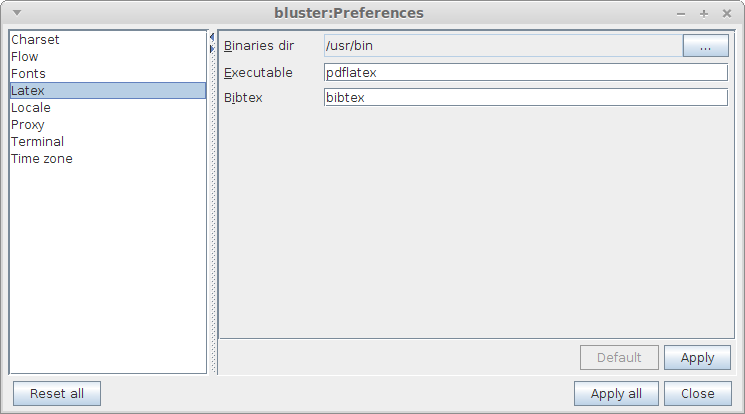
\includegraphics[width=8.0cm]{images/latex_preferences.png}
  \caption{Latex preferences}
  \label{latex_preferences}
\end{figure}

%%%%%%%%%%%%%%%%%%%%%%%%%%%%%%%%%%%
% Copyright (c) 2009-2012 by the University of Waikato, Hamilton, NZ. 
% This work is made available under the terms of the 
% Creative Commons Attribution-ShareAlike 4.0 license,
% http://creativecommons.org/licenses/by-sa/4.0/.
%
% Version: $Revision$

\begin{thebibliography}{999}
	% to make the bibliography appear in the TOC
	\addcontentsline{toc}{chapter}{Bibliography}

    % references
	\bibitem{adams}
		\textit{ADAMS} -- Advanced Data mining and Machine learning System \\
		\url{https://adams.cms.waikato.ac.nz/}{}
		
	\bibitem{heatmap}
		\textit{Heat map} -- WikiPedia article \\
		\url{http://en.wikipedia.org/wiki/Heat_map}{}

\end{thebibliography}


\end{document}
